\documentclass[a4paper,12pt]{article}

%%% Работа с русским языком
\usepackage{cmap}					% поиск в PDF
\usepackage{mathtext} 				% русские буквы в формулах
\usepackage[T2A]{fontenc}			% кодировка
\usepackage[utf8]{inputenc}			% кодировка исходного текста
\usepackage[english,russian]{babel}	% локализация и переносы
\usepackage{indentfirst}
\frenchspacing


%%% Дополнительная работа с математикой
\usepackage{amsmath,amsfonts,amssymb,amsthm,mathtools} % AMS
\usepackage{icomma} % "Умная" запятая: $0,2$ --- число, $0, 2$ --- перечисление

%% Номера формул
%\mathtoolsset{showonlyrefs=true} % Показывать номера только у тех формул, на которые есть \eqref{} в тексте.
%\usepackage{leqno} % Нумерация формул слева

%% Свои команды
\DeclareMathOperator{\sgn}{\mathop{sgn}}

%% Перенос знаков в формулах (по Львовскому)
\newcommand*{\hm}[1]{#1\nobreak\discretionary{}
	{\hbox{$\mathsurround=0pt #1$}}{}}

%%% Работа с картинками
\usepackage{graphicx}  % Для вставки рисунков
\graphicspath{{images/}}  % папки с картинками
\setlength\fboxsep{3pt} % Отступ рамки \fbox{} от рисунка
\setlength\fboxrule{1pt} % Толщина линий рамки \fbox{}
\usepackage{wrapfig} % Обтекание рисунков текстом

%%% Работа с таблицами
\usepackage{array,tabularx,tabulary,booktabs} % Дополнительная работа с таблицами
\usepackage{longtable}  % Длинные таблицы
\usepackage{multirow} % Слияние строк в таблице

%%% Теоремы
\theoremstyle{plain} % Это стиль по умолчанию, его можно не переопределять.
\newtheorem{theorem}{Теорема}[section]
\newtheorem{proposition}[theorem]{Утверждение}

\theoremstyle{definition} % "Определение"
\newtheorem{corollary}{Следствие}[theorem]
\newtheorem{problem}{Задача}[section]

\theoremstyle{remark} % "Примечание"
\newtheorem*{nonum}{Решение}

%%% Программирование
\usepackage{etoolbox} % логические операторы

%%% Страница
\usepackage{extsizes} % Возможность сделать 14-й шрифт
\usepackage{geometry} % Простой способ задавать поля
\geometry{top=15mm}
\geometry{bottom=20mm}
\geometry{left=20mm}
\geometry{right=20mm}
%
%\usepackage{fancyhdr} % Колонтитулы
% 	\pagestyle{fancy}
%\renewcommand{\headrulewidth}{0pt}  % Толщина линейки, отчеркивающей верхний колонтитул
% 	\lfoot{Нижний левый}
% 	\rfoot{Нижний правый}
% 	\rhead{Верхний правый}
% 	\chead{Верхний в центре}
% 	\lhead{Верхний левый}
%	\cfoot{Нижний в центре} % По умолчанию здесь номер страницы

\usepackage{setspace} % Интерлиньяж
%\onehalfspacing % Интерлиньяж 1.5
%\doublespacing % Интерлиньяж 2
%\singlespacing % Интерлиньяж 1

\usepackage{lastpage} % Узнать, сколько всего страниц в документе.

\usepackage{soul} % Модификаторы начертания

\usepackage{hyperref}
\usepackage[usenames,dvipsnames,svgnames,table,rgb]{xcolor}
\hypersetup{				% Гиперссылки
	unicode=true,           % русские буквы в раздела PDF
	pdftitle={Заголовок},   % Заголовок
	pdfauthor={Автор},      % Автор
	pdfsubject={Тема},      % Тема
	pdfcreator={Создатель}, % Создатель
	pdfproducer={Производитель}, % Производитель
	pdfkeywords={keyword1} {key2} {key3}, % Ключевые слова
	colorlinks=true,       	% false: ссылки в рамках; true: цветные ссылки
	linkcolor=violet,          % внутренние ссылки
	citecolor=black,        % на библиографию
	filecolor=orange,      % на файлы
	urlcolor= blue           % на URL
}

\usepackage{csquotes} % Еще инструменты для ссылок

%\usepackage[style=authoryear,maxcitenames=2,backend=biber,sorting=nty]{biblatex}

\usepackage{multicol} % Несколько колонок

\usepackage{tikz} % Работа с графикой
\usepackage{pgfplots}
\usepackage{pgfplotstable}

% Use more than one optional parameter in a new commands
\usepackage{xargs}

% to-do notes
\usepackage[colorinlistoftodos,prependcaption,textsize=tiny]{todonotes}
\newcommandx{\improvement}[2][1=]{\todo[linecolor=Plum,backgroundcolor=Plum!25,bordercolor=Plum,#1]{#2}}

\renewcommand{\phi}{\varphi}
\renewcommand{\epsilon}{\varepsilon}
\usepackage[backend=biber]{biblatex}

\addbibresource{lit.bib}

\makeatletter
\let\@fnsymbol\@arabic
\makeatother


\title{Тензорная декомпозиция и прогноз для набора временных рядов}
\author{Сёмкин Кирилл$^{1}$ \\ {\footnotesize $^{1}$semkin.ki@phystech.edu} \and Вадим Стрижов$^{2}$ \\ {\footnotesize $^{2}$vadim.swifton@gmail.com}}
\date{}


\begin{document}
	
	\maketitle
	
	\begin{abstract}
		
		Декомпозиция временного ряда часто применяется для получения его структуры: разложения на простые и/или интерпретируемые составляющие, выявление периодичности, избавление от шума и т.д. В случае же набора нескольких рядов игнорирование взаимосвязей между ними может приводить к некачественным и ложным разложениям и предсказаниям. В данной работе предлагается метод декомпозиции, учитывающий фактор связанности и основанный на классическом методе SSA (Гусеница) и тензорных разложениях, а также способ прогноза будущих значений ряда. Предложенный подход сравнивается с похожим mSSA, основанным на матричных разложениях, в математических свойствах и при обработке синтетических и реальных данных (потребление электроэнергии, акселерометрия).
		
	\end{abstract}
	
	\textit{Ключевые слова}: {\small декомпозиция, прогноз, SVD, SSA, тензорные разложения}.
	
	
	\section*{Введение}\label{Intro}
	
		Выявление структуры временного ряда --- краеугольная задача математического прогнозирования. Любой метод, независимо от его назначения и цели: предсказание, восстановление пропусков в данных, декомпозиция и т.д., напрямую или косвенно имеет свои предположения насчёт этой структуры. Например, модели стационарных временных рядов (\cite{Box_Jenkins_methodology}, \cite{hamilton1994time}) предполагают рассматриваемый случайный процесс стационарным в широком смысле. Применяемые методы регрессионного анализа (\cite{3b1355aedd1041f1853e609a410576f3}, \cite{Greene2003Econometric}, \cite{enders2010applied})  рассматривают время в качестве независимых переменных (регрессов) и вводят параметрическую модель $ f(\mathbf{\Theta}, t) $, отражающую структуру ряда. Также часто применяются методы на основе динамических систем (\cite{ecfb9dc578be43ae9ee8fc88b8ff9151}, \cite{chen2018neural}, \cite{Tsonis2018}) , предполагающие существование таковой и порождающей наблюдаемый временной ряд напрямую или косвенно. Один из подходов такого типа --- \textbf{SSA}, широко применяется в задачах прогнозирования и разложения на составляющие сигналы.
		
		Классическая постановка задачи декомпозиции временного ряда состоит в его разложении на сезонную, циклическую, тренд и шумовую составляющие. Циклическую и трендовую часть часто объединяют в одну компоненту. Также разложение может быть аддитивным (исходный ряд --- сумма компонент) или мультипликативным (исходный ряд --- произведение компонент). Существует большое количество методов разложения на основе техники скользящего среднего MA (\cite{enders2010applied}, \cite{x11}, \cite{cleveland90}), подбирая сначала авторегрессионную трендовую компоненту, затем усреднением остатка ряда получается сезонная компонента. Данный класс приёмов активно используется в эконометрике и финансах. Также возможно разложение сигнала в ряд фурье по гармоникам или полиномам, и связанные с ним более продвинутые методы (вейвлет преобразование и др.). Данное разложение удобно для амплитудно-частотного анализа сигнала и его фильтрации, но оно имеет недостаток фиксированного базиса функций, по которой раскладывается ряд. Метод SSA же позволяет получить адаптивный базис разложения, связанный с пространством скрытой динамической системы, порождающей наблюдаемый сигнал. Если полученные базисные векторы возможно разделить на группы, отвечающие своему порождаемому сигналу, то мы получаем желаемую декомпозицию исходного ряда. Также данный базис возможно использовать для построения прогноза, что будет показано ниже.
		
		В случае же набора временных рядов, связанных единой системой (например, показания акселерометра и гироскопа; количество реагентов типа А и B при протекании их совместной реакции и т.д.), их разложение порознь обычными методами скорей всего ни отразит их общей структуры, ни даст качественных, интерпретируемых компонент. Для решения данной проблемы существует простая модификация 'Гусеницы' - \textbf{mSSA}, описание которой будет приведено ниже. Она успешно применяется на практике: например, изучение фазовой синхронизации \cite{PhysRevE.84.036206} или восстановление пропусков в временных рядах. \cite{agarwal2020multivariate}.
		
	    В данной работе вводится ещё одна модификация: \textbf{tSSA}, в которой предлагается использовать мощь тензорных разложений вместо матричных. В большинстве своём для них нет быстрых прямых алгоритмов (например, одно вычисление тензорного ранга - NP-трудная задача, см. \cite{HASTAD1990644}), но существуют достаточно быстрые приближённые, что в случае больших выборок будет вычислительно эквивалентно скорости матричных методов. С другой стороны, представление временных рядов в виде тензора и его декомпозиция потенциально более выразительна и способна  выявить более тонкие взаимосвязи между рядами. Применение и исследование данного метода можно найти в \cite{6661921}, \cite{6834801}, где авторы сворачивают одномерный сигнал ЭКГ активности мозга в трёхмерный тензор и получают его разложение по IMFs (intrinsic mode functions) определённых частот. В работе \cite{app7040418} авторы применяют ту же технику но для анализа сигнала отклика механических систем, а также предлагают сведение задачи тензорного разложения к задаче выпуклой оптимизации. В работах \cite{10122507} и \cite{FU2023115} исследователи работают с \href{https://en.wikipedia.org/wiki/Hyperspectral_imaging}{гиперспектральными изображениями}, которые уже по своей природе представляются в виде многомерных массивов, и тензорное разложение позволяет учесть не только взаимодействие спектральных каналов изображения, но также и пространственных. Метод успешно применяется для сегментации изображений земной поверхности. 
	    
	    Далее будет дано математическое описание алгоритмов mSSA и tSSA, их особенности и сравнение в подходах к декомпозиции многомерных рядов. Также будет описан метод построения прогноза для метода mSSA, основанный на способе прогнозирования в классическом SSA. Похоже будет введено прогнозирование и в tSSA. После данные методы тестируются на разложении и предсказании набора синтетических рядов, а также на реальных данных: потребление электроэнергии частным домохозяйством в течении года и данными акселерометра движущегося пешехода. Анализируется ошибка, возникающая при разложении рядов, интерпретируемость разложения, качество предсказания на отложенных значениях выборки. 
	    
	    \section*{Теоретическая часть}
	    
	    	Пусть имеем набор временных рядов $ \{x_i(t_j)\}_{i = 1}^{m} $, где сетка по времени $ t_j \in \overrightarrow{1, N} $. Стоит задача разложения временных рядов на аддитивные компоненты: 
	    	
	    	\begin{gather*}
	    		x_1(t) = f_1(t) + f_2(t) + \ldots + f_{n_1}(t) \\
	    		x_2(t) = g_1(t) + g_2(t) + \ldots + g_{n_2}(t) \\
	    			   ...
	    	\end{gather*}
	    	
	    	Формулировка задачи слишком общая, ведь таких разложений для произвольной функции можно построить сколь угодно много и каким угодно способом: можно раскладывать по индикаторным функциям (любую измеримую функцию можно так разложить), в ряды Фурье и т.д. Мы же будем полагаться на свойства вводимых далее методов обработки временных рядов для поиска этого разложения, а также для построения прогноза.
	    
	    	\subsection*{Метод SSA}
	    	
	    	Пусть имеем пока один времнной ряд. Подход "Гусеницы" предполагает наличие некоторой динамической системы, порождающей наблюдаемый ряд, и опирается на теорему Такенса об аппроксимации многообразия, в котором лежат траектории системы, так называемыми \textit{векторами временных задержек} (\cite{citeulike:2735031}). Для построения этих векторов выбирается длина окна $ L $, далее это окно "скользит" по временному ряду, выделяя в нём $ L $ значений (см. рис.\ref{pic:hankel_build} ). Формально k-ый вектор задержек есть $ \mathbf{x}_k = ( x(t_k) \  x(t_{k+1}) \  \ldots \  x(t_{k + L - 1}) ) $. Далее данные вектора собираются в матрицу $ T_{ij} $ по столбцам, у которой в результате все антидиагональные элементы $ i + j = const $ равны. Такие матрицы называются \textit{ганкелевыми}, а в терминах временных рядов матрица $ T $ называется \textit{траекторной} или \textit{матрицей задержек}.
	    	
	    	\begin{figure}
	    		\centering
	    		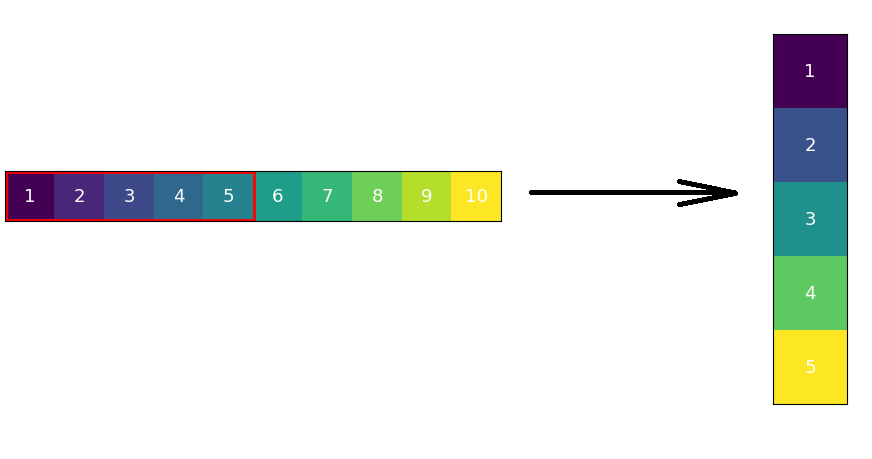
\includegraphics[width=0.6\textwidth, keepaspectratio]{../figs/first_round}
	    		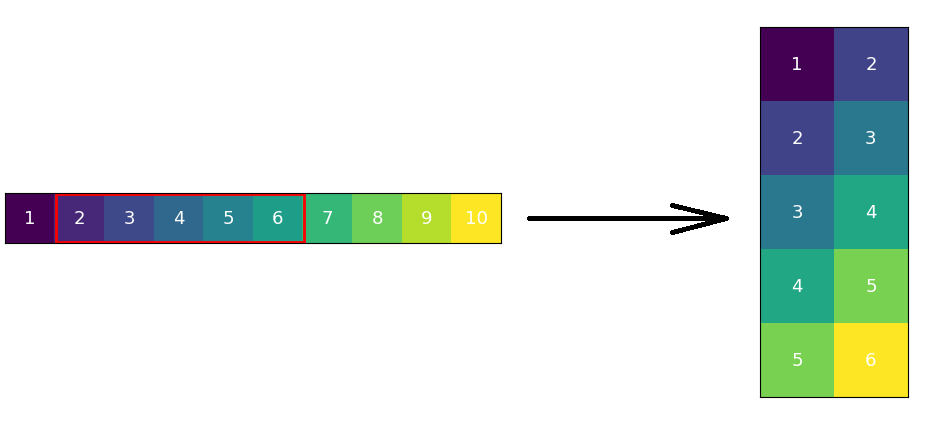
\includegraphics[width=0.6\textwidth, keepaspectratio]{../figs/second_round.png}
	    		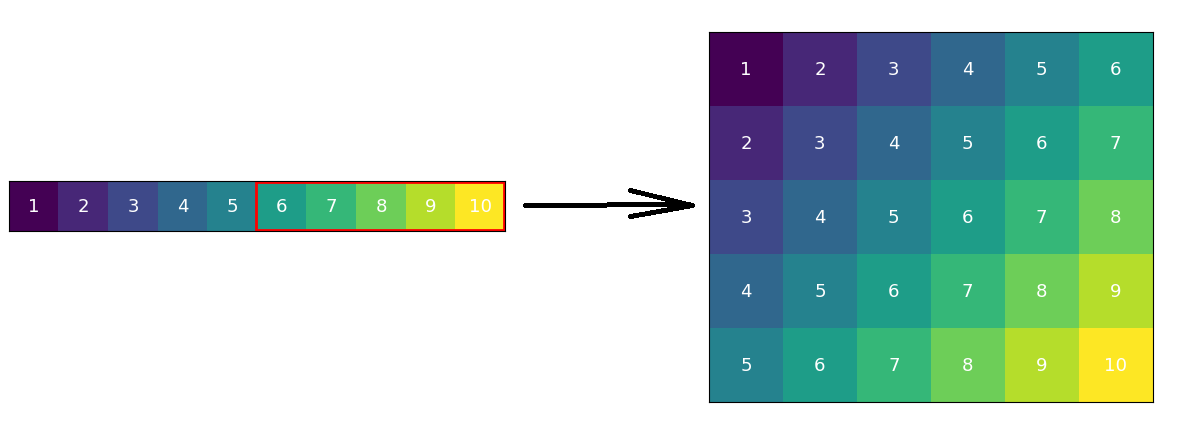
\includegraphics[width=0.6\textwidth, keepaspectratio]{../figs/last_round.png}
	    		\caption{Построение ганкелевой матрицы}\label{pic:hankel_build}
	    	\end{figure}
	    	
	    	Далее к матрице применяется SVD-разложение $ T = \sum\limits^{r} \sigma_i \mathbf{u}_i \mathbf{v}_i $ (знак транспонирования для $ \mathbf{v}_i $ опускается), получая таким образом тот самый адаптивный ортонормированный базис $ \{\mathbf{u}_i\}_{i=1}^r $ в пространстве векторов задержек. Компоненты с малыми $ \sigma_i $ интерпретируются как шумовые.
	    	
	    	Для декомпозиции исходного ряда предлагается следующее: пусть $ x(t) = f_1(t) + f_2(t) $ и пусть мы построили ганкелевы матрицы $ X_1, X_2 $ для $ f_1(t) $ и $ f_2(t) $, тогда $ T = X_1 + X_2 $. Как известно, SVD-разложение матриц единственно (разложение по ортонормированному базису), т.е. для матриц $ X_1 $ и $ X_2 $ это разложение по тем же базисам $ \{\mathbf{u}_i\}_{i=1}^r, \  \{\mathbf{v}_i\}_{i=1}^r $. Главное предположение здесь --- возможность разделить эти базисы на две \underline{непересекающиеся} группы:  $ ( \{\mathbf{u}^1_i\}_{i=1}^{r_1}, \, \{\mathbf{v}^1_i\}_{i=1}^{r_1} ) $ и $ ( \{\mathbf{u}^2_i\}_{i=1}^{r_2}, \, \{\mathbf{v}^2_i\}_{i=1}^{r_2} ) $, где $ r_1 + r_2 = r $. Тогда возможно выделить декомпозицию исходного ряда из его сингулярного разложения:
	    	
	    	\begin{equation*}
	    		 T = \sum\limits_i^{r} \sigma_i \mathbf{u}_i \mathbf{v}_i = \sum\limits_i^{r_1} \sigma_i^1 \mathbf{u}_i^1 \mathbf{v}_i^1 + \sum\limits_i^{r_2} \sigma_i^2 \mathbf{u}_i^2 \mathbf{v}_i^2 = X_1 + X_2
	    	\end{equation*}
	    	
	    	Получив $ X_1, X_2 $ можно однозначно восстановить $ \{f_1(t_j)\}, \{f_2(t_j)\} $, для этого достаточно взять первый столбец и последнюю строки в этих матрицах и соединить в один вектор друг за другом --- это просто следует из способа построения матриц векторов задержек и их ганкелевой структуры. Таким же образом можно разделять спектральное разложение на большее число групп и по той же процедуре извлекать составляющие сигнала, если гипотеза возможности такого разделения верна.
	    	
	    	Вводимое предположение имеет следующий смысл: т.к. вектора задержек для $ f_1(t) $ и $ f_2(t) $ лежат в ортогональных друг другу пространствах, порождённых $ \{\mathbf{u}^1_i\}_{i=1}^{r_1} $ и $ \{\mathbf{u}^2_i\}_{i=1}^{r_2} $, то и исходные вектора задержек двух рядов ортогональны друг другу:
	    	
	    	\[
	    		 f_1(t_i) f_2(t_i) + \ldots + f_1(t_{i + L - 1}) f_2(t_{i + L - 1}) = <f_{1, L}, f_{2, L}> = 0, \  \forall i \in \overrightarrow{1, N - L + 1}
	    	\]
	    	
	    	 С точки зрения динамических систем, между векторами задержек и многообразием траекторий скрытой системы существует диффеоморфизм, таким образом существование предполагаемого разделение говорит о разложимости скрытого многообразия в прямую сумму подпространств.
	    	
	    	Как показано в подробной книге о методе SSA \cite{ecfb9dc578be43ae9ee8fc88b8ff9151}, предложенным способом невозможно строго разделить даже достаточно простые сигналы. Тем не менее, в асимптотическом приближении $ N \to \infty, L \to \infty $ они разделяются, т.е. их корреляция в этом случае $ <f_{1, L}, f_{2, L}> \to 0 $, см. табл.\ref{tab:asympt_devis}. Также там показано, что если $ \exists \tilde{L}: \forall L > \tilde{L} \hookrightarrow rank(T) = r = const $, то исходный ряд в точности описывается авторегрессионной моделью.
	    	
	    	\begin{table}[h]
	    		\centering
	    		\caption{Асимптотическая разделимость компонент (Golyandina)}\label{tab:asympt_devis}
	    		\begin{tabular}{|c|c|c|c|c|c|}
	    			\hline
	    			& const & cos & exp & exp (cos) & ak + b \\ \hline
	    			const     & -     & +   & +   & +         & -      \\ \hline
	    			cos       & +     & +   & +   & +         & +      \\ \hline
	    			exp       & +     & +   & +   & +         & +      \\ \hline
	    			exp (cos) & +     & +   & +   & +         & +      \\ \hline
	    			ak + b    & -     & +   & +   & +         & -      \\ \hline
	    		\end{tabular}
	    	\end{table}
	    	
	    	Далее, любые данные содержат в себе ошибки (шум, неточности вычислений и т.д.), поэтому даже строго разделяемые ряды на практике не получится идеально декомпозировать. Поэтому применяется простая процедура: полученные в ходе разделения главных компонент $ X_1, X_2 $ \textit{ганкелизуются}, т.е. каждая антидиагональ матриц усредняется и заменяется на это среднее. Таким образом оценивать полученную декомпозицию можно по получившейся невязке. \improvement{втавить оценку ошибки такого приближения}
	    	
	    	%TODO: втавить оценку ошибки такого приближения
	    	
	    	Что касается поиска группировки на основе SVD разложения, здесь не существует общего алгоритма. Часто для разделения главных компонент используют \textit{относительную близость спектральных чисел}, группируя факторы по их близости друг к другу. В той же \cite{ecfb9dc578be43ae9ee8fc88b8ff9151} есть  обоснования такого подхода для нескольких классов функций.	    	
	    	
	    	
			\subsection*{Метод mSSA. Декомпозиция}
			
			Пусть теперь имеем $ m $ временных рядов $ \{x_i(t_j)\}_{i = 1}^{m} $, где $ t_j \in \overrightarrow{1, N} $. Предполагая ту же гипотезу о природе порождения этих сигналов, будет действовать похожим на SSA способом. Для этого опять выбираем длину окна $ L $ и строим траекторные матрицы для каждого ряда $ T_1, T_2, \ldots , T_m  $. Теперь конкатенируем все матрицы в одну $ T = [T_1 \  T_2 \ldots T_m] $, которую далее раскладываем с помощью SVD:
			
			\begin{equation*}
				T = \sum\limits_i^{r} \sigma_i \mathbf{u}_i \mathbf{v}_i \Leftrightarrow \begin{cases}
					T_1 = \sum\limits_i^{r} \sigma_i \mathbf{u}_i \mathbf{v}_i^1 \\
					T_2 = \sum\limits_i^{r} \sigma_i \mathbf{u}_i \mathbf{v}_i^2 \\
					\ldots \\
					T_m = \sum\limits_i^{r} \sigma_i \mathbf{u}_i \mathbf{v}_i^m
				\end{cases}
			\end{equation*}
			
			Здесь каждая главная компонента в пространстве строк $ \mathbf{v}_i $ представляется в виде конкатенации: $ \mathbf{v}_i = (\mathbf{v}_i^1 \ldots \mathbf{v}_i^m) $. Т.о. получаем некоторое разложение траекторных матриц, которое не является SVD-разложением в общем случае (т.к. компоненты $ \mathbf{v}_i^k $ не обязаны быть ортогональны между собой). Тем не менее базис столбцов у всех сигналов одинаковый $ \{\mathbf{u}_i\}_{i=1}^r $ и ортонормированный, "сингулярные" числа тоже одинаковые. В итоге общее столбцовое пространство связывает траекторные матрицы каждого ряда и учитывает их общую природу порождения.
			
			Дальнейший ход действий для декомпозиции аналогичен методу SSA. Можно рассматривать разложение каждой траекторной матрицы отдельно, но т.к. все они имеют общий набор $ \{\sigma_i \} $, и группировка главных компонент часто делается на их основе, то разделение на группы происходит одинаковое для всех траекторных матриц. Получаем итоговое разложение каждого сигнала в виде:
			
			\begin{gather*}
				x_1(t) = \hat{f}_1(t) + \hat{f}_2(t) + \ldots + \hat{f}_{n}(t) \\
				x_2(t) = \hat{g}_1(t) + \hat{g}_2(t) + \ldots + \hat{g}_{n}(t) \\
				... \\
				x_m(t) = \hat{h}_1(t) + \hat{h}_2(t) + \ldots + \hat{h}_{n}(t)
			\end{gather*}
			
			\subsection*{Метод tSSA}\label{tSSA_sec}
			
			Данный подход основан на сборке того же набора рядов $ \{x_i(t_j)\}_{i = 1}^{m} $ в тензор и применения уже \textit{тензорного} разложения вместо рассматриваемого до этого SVD. Сразу отметим, что способов упаковки и разложений для тензоров можно предложить огромное количество (для базового ознакомления можно, например, обратиться к \cite{rabanser2017introduction}; также см. предлагаемые работы в \nameref{Intro}), являясь ещё скудно изученной областью в приложении к временным рядам.
			
			 В данной работе предлагается вдохновлённый классическим SSA способ получения \textit{траекторного тензора} $ \mathbf{T} $: как и в mSSA, строятся траекторные матрицы для каждого ряда $ T_1, \ldots, T_m $, после чего данные матрицы состыковываются друг с другом по третьему измерению (индексу) тензора. Т.о. измерениям $ \mathbf{T} $ соответствуют столбцы и строки временных задержек, а также номер сигнала. Далее, к полученному тензору применяется \textit{каноническое разложение} (Canonical polyadic decomposition, CPD), т.к. нам важно сохранить структуру суммы одноранговых факторов (см. рис.\ref{pic:cpu_dec}).
			 
			 С математической точки зрения это выглядит так:
			 
			 \begin{equation}\label{eq:tSSA_decomp}
			 	\mathbf{T} = \sum\limits_i^{r} \mathbf{a}_i \otimes \mathbf{b}_i \otimes \mathbf{c}_i \Leftrightarrow \begin{cases}
			 		T_1 = \sum\limits_i^{r} \mathbf{c}_i[1] \cdot \mathbf{a}_i  \mathbf{b}_i  \\
			 		T_2 = \sum\limits_i^{r} \mathbf{c}_i[2] \cdot \mathbf{a}_i  \mathbf{b}_i \\
			 		\ldots \\
			 		T_m = \sum\limits_i^{r} \mathbf{c}_i[m] \cdot \mathbf{a}_i  \mathbf{b}_i 
			 	\end{cases}
			 \end{equation}
			 
			 \begin{figure}[h]
			 	\centering
			 	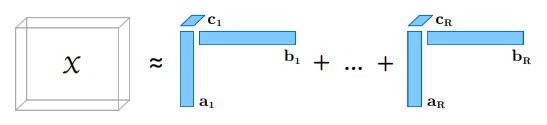
\includegraphics[width=0.6\textwidth, keepaspectratio]{../figs/cpu_decomp}
			 	\caption{Иллюстрация канонического разложения}\label{pic:cpu_dec}
			 \end{figure}
			 
			 Здесь записано разложение исходного тензора в сумму тензорных произведений набора векторов $ \mathbf{a}_i, \mathbf{b}_i, \mathbf{c}_i $, которые можно для удобства состыковать в матрицы $ A, B, C $. Если зафиксировать третий индекс, то получим разложение каждой траекторной матрицы $ T_i $, где $ \mathbf{c}_i[k] $ --- это $ k $-ая компонента вектора $ \mathbf{c}_i $. Таким образом разложение происходит по одному базису как для столбцов, так и для строк у каждой матрицы задержек! Роль же сингулярных чисел играют строки матрицы $ C $. Дальнейший ход действий для получения декомпозиции аналогичен SSA.
			 
			 Полученное разложение обладает \textit{рядом преимуществ} по сравнению с mSSA: теперь имеем общий базис как у столбцов, так и у строк матриц $ T_i $, что ещё сильнее связывает каждый сигнал; тем более строки у $ T_i $ - это те же вектора задержек, только другой размерности, поэтому странно раскладывать их для каждой $ T_i $ по своему базису, если столбцы раскладываются по одному. Также данное разложение более гибкое, т.к. для каждой матрицы задержки имеется свой набор $ \mathbf{c}_i[k], \,  k \in \overrightarrow{1, r} $ "сингулярных" чисел, что позволяет каждому сигналу подстроиться под базисные векторы индивидуально. Таким образом каждую траекторную матрицу можно раскладывать также индивидуально, что было затруднительно в mSSA. Ещё одним положительным моментом является свойство CPD-разложения: при весьма необременительных условиях оно единственно, что сводит поиск любого разложения траекторных матриц в виде (\ref{eq:tSSA_decomp}) к CPD-разложению тензора $ \mathbf{T} $.
			 
			 
			 Тем не менее есть и некоторые недостатки по сравнению с матричным разложением: теперь базисы в пространстве столбцов не составляют ортогональную систему (чего не скажешь о mSSA), в пространстве строк аналогично (но у mSSA та же проблема). Также их необходимо нормировать для преемственности с предыдущими методами, нормы векторов скорректируют изначальные "сингулярные" числа (далее по умолчанию предполагаем нормированность). Ещё эти числа могут быть отрицательными, что уменьшает их интерпретируемость и помощь в группировке. Тем не менее теперь можно отбрасывать те из них, что будут \textit{малы по модулю}.
			 
			 
			 \subsection*{Построение прогноза в рассмотренных методах}
			 
			 Опишем метод построения прогноза в модели \textbf{SSA}. Допустим последнее известное значение ряда $ x_T $, хотим построить прогноз на $ k $ шагов вперёд.
			 
			 Считаем, что ширина окна $ L $ для векторов задержки выбрана достаточная, а также имеем достаточное количество измерений ряда $ N $, чтобы выполнялась теорема Такенса. Тогда динамика векторов задержек диффеоморфна динамике скрытой порождающей наш ряд системе, т.е. все её траектории лежат в некотором многообразии $ M \subset \mathcal{L}_r $, где $ \mathcal{L}_r = Lin(\mathbf{u}_1, \ldots, \mathbf{u}_r) $ - линейная оболочка ортонормированной системы, найденной с помощью SVD разложения. Введём матрицу $ U = [\mathbf{u}_1, \ldots, \mathbf{u}_r] $.
			 
			 Теперь рассмотрим вектор задержки $ \mathbf{x} = (x_{T + k - L + 1} \ldots x_T \ldots x_{T + k}) $; разделим его на неизвестную (последние $ k $ компонент) $ \mathbf{x}_{pr} $ и известную (оставшиеся компоненты) $ \mathbf{x}_{kn} $ часть. Аналогично разделим матрицу $ U $ на $ U_{kn} $ (первые $ L - k $ строк) и $ U_{pr} $ (последние $ k $ строк). Имеем $ \mathbf{x} \in M \subset \mathcal{L}_r $, т.е. этот вектор раскладывается по базису $ \{\mathbf{u}_i\}^r $, а значит $ \exists! \, \boldsymbol{\lambda} \in \mathbb{R}^r $ т.ч.:
			 
			 \begin{equation}\label{eq:pred_main}
			 	\mathbf{x} = U \boldsymbol{\lambda} \Leftrightarrow \begin{cases*}
			 		\mathbf{x}_{kn} = U_{kn} \boldsymbol{\lambda} \\
			 		\mathbf{x}_{pr} = U_{pr} \boldsymbol{\lambda}
			 	\end{cases*}
			 \end{equation}
			 
			 Это основное уравнение для получения предсказания, на его основе будет построен прогноз и в tSSA. Пока что заметим: из ортогональности $ U $ можно явно получить $ \boldsymbol{\lambda} = U^T \mathbf{x} $. Подставим это в выражение для $ \mathbf{x}_{pr} $:
			 
			 \begin{gather}
			 	\mathbf{x}_{pr} = U_{pr} U^T \mathbf{x} =  U_{pr} (U_{kn}^T \, U_{pr}^T) (\mathbf{x}_{kn} \, \mathbf{x}_{pr})^T = U_{pr} (U_{kn}^T \mathbf{x}_{kn} + U_{pr}^T \mathbf{x}_{pr}) \nonumber \\
			 	\mathbf{x}_{pr} (I -  U_{pr}  U_{pr}^T) =  U_{pr}  U_{kn}^T \mathbf{x}_{kn} \nonumber \\
			 	\mathbf{x}_{pr} = (I -  U_{pr}  U_{pr}^T)^{-1} U_{pr}  U_{kn}^T \mathbf{x}_{kn}\label{eq:pred_sol_1}
			 \end{gather}
			 
			 Последнее выражение верно при условии обратимости соответствующего члена. \smallskip
			 
			 Проанализируем ещё раз систему из (\ref{eq:pred_main}): найти $ \boldsymbol{\lambda} $ можно только из выражения для $ \mathbf{x}_{kn} $; сделав это, мы можем получить желаемый прогноз $ \mathbf{x}_{pr} $ из той же (\ref{eq:pred_main}). Мы знаем, что $ rank(U) = r $ и того же хочется для $ U_{kn} $, ведь в противном случае ядро $ Ker(U_{kn}) \not= \{0\} $ и даже если решение для $ \boldsymbol{\lambda} $ есть, то оно не единственно и может быть сколь угодно большим: $ \boldsymbol{\lambda} = \boldsymbol{\lambda}_{particular} + \mathbf{c} \cdot Ker(U_{kn}) $, где $ \mathbf{c} $ --- вектор произвольных констант. А в этом случае сколь угодно большим и неопределённым может быть и $ \mathbf{x}_{pr} $, что плохо с точки зрения интерпретируемости (с другой стороны можно привлечь здесь идеи байесовского анализа и ввести априорное распределение на вектор $ \mathbf{c} $, далее по имеющимся данным строить апостреорное распределение для $ \mathbf{x}_{pr} $ и делать прогноз, но это не тема данной работы). $ rank(U_{kn}) $ определяется тем, где находятся линейно-независимые строки в матрице $ U $: хочется, чтобы все они находились как можно выше в $ U $, чтобы $ U_{kn} $ была полного ранга даже для больших горизонтах прогнозирования $ k $. Пусть в $ U $ нашли такой набор строк, причём наибольший номер строки в этом наборе получился $ K $. Тогда понятно, что, во-первых, $ K \ge r $, во-вторых, однозначный прогноз можно получить только для $ k \le L - K \le L - r $.
			 
			 Теперь обсудим существование решения для $ \boldsymbol{\lambda} $. Если его нет, то нет и решения для $ \mathbf{x} $, но мы предполагаем, что есть многообразие $ M \subset \mathcal{L}_r $, в котором лежат траектории векторов задержек, и они должны быть определены для любых моментов времени. Вектор $ x $ содержит в себе часть вектора задержки и если решения для $ \boldsymbol{\lambda} $ нет, то вообще не существует точки траектории, которую потенциально представляет $ \mathbf{x} $ (потенциально --- потому что вообще он не определён полностью), и это противоречие. Таким образом, если все наши предположения, продиктованные теорией Такенса, выполнены, мы можем рассчитывать на \textit{однозначно определённый прогноз} временного ряда. Отсюда же следует условие для обратимости матрицы $ I -  U_{pr}  U_{pr}^T $.
			 
			 Ещё одно замечание: из всего вышесказанного следует, что можно получать прогнозы разными способами, ведь $ k $ можно выбирать любым от $ 1 $ до $ L - K $. Из однозначности этого прогноза для всех таких $ k $ следует, что все эти способы должны приводить к одному результату. Для вычисления $ \mathbf{x}_{pr} $ нужно обратить матрицу размера $ k \times k $ и перемножить два раза вектор на матрицу. Т.к. обращение в общем случае достаточно трудоёмкая операция, то рекомендуется строить прогноз для $ k = 1 $ столько раз, сколько нужно.
			 
			 Из всего вышесказанного, нетрудно понять, как строиться прогноз в \textbf{mSSA}: здесь мы также имеем ортонормированный базис в пространстве траекторий векторов задержек $ \{\mathbf{u}_i\}^r $, единый для всех сигналов. Таким образом поступаем аналогичным SSA способом для каждого имеющегося временного ряда.
			 
			 Для \textbf{tSSA} ситуация несколько иная. Здесь роль $ U $ играет матрица $ A $ (см. раздел выше), которая полного ранга, но не ортогональная (но все столбцы нормированы в единицу по построению). Соответственно уравнение (\ref{eq:pred_main}) здесь выглядит:
			 
			 \begin{equation}\label{eq:main_pred_for_A}
			 	\mathbf{x} = A \boldsymbol{\lambda} \Leftrightarrow \begin{cases*}
			 		\mathbf{x}_{kn} = A_{kn} \boldsymbol{\lambda} \\
			 		\mathbf{x}_{pr} = A_{pr} \boldsymbol{\lambda}
			 	\end{cases*}
			 \end{equation}
			 
			 Вышеизложенная теория полностью переносится на этот случай, за исключением того, что выразить $ \boldsymbol{\lambda} $ через $ A $ просто не получится, но тем не менее решение должно существовать для любого горизонта прогнозирования $ k \le L - K $.
			 
			 Разложим $ A $ через SVD: $ A = U \Sigma V^T $, а также выразим $ \boldsymbol{\lambda} $ через псевдообратную к $ A $: $ \boldsymbol{\lambda} = (A^T A)^{-1} A^T \mathbf{x} $ --- в наших условиях это и есть решение СЛАУ выше (в общем случае --- решение только в смысле наименьших квадратов). Проводя абсолютно аналогичные (\ref{eq:pred_sol_1}) операции, получим:
			 
			 \begin{equation*}
			 	(I - A_{pr} (A^T A)^{-1} A^T A_{pr}^T) \mathbf{x}_{pr} = A_{pr} (A^T A)^{-1} A^T A_{kn}^T \mathbf{x}_{kn}
			 \end{equation*}
			 
			 Также проведя простые операции с SVD разложением для $ A $, получим следующее:
			 
			 \begin{gather*}
			 	A_{pr} (A^T A)^{-1} A^T A_{pr}^T = U_{pr} (U^T V \Sigma) U_{pr}^T \\
			 	A_{pr} (A^T A)^{-1} A^T A_{kn}^T = U_{pr} (U^T V \Sigma) U_{kn}^T
			 \end{gather*}
			 
			 Откуда получаем:
			 
			 \begin{equation}
			 	(I - U_{pr} (U^T V \Sigma) U_{pr}^T) \mathbf{x}_{pr} = U_{pr} (U^T V \Sigma) U_{kn}^T \mathbf{x}_{kn}
			 \end{equation}
			 
			 Получаем очень похожее на (\ref{eq:pred_sol_1}) выражение, в котором дополнительно фигурирует невырожденная квадратная матрица $ U^T V \Sigma $ размера $  r \times r$ ($ r $ --- тензорный ранг). Домножая слева на обратную матрицу, можно выразить $ \mathbf{x}_{pr} $, но, т.к. на практике достаточно и проще всего делать прогноз на $ k = 1 $, то можно из (\ref{eq:main_pred_for_A}) выразить $ \boldsymbol{\lambda} = (A_{kn}^T A_{kn})^{-1} A_{kn}^T \mathbf{x}_{kn} $, тогда получим:
			 
			 \begin{equation}
			 	\mathbf{x}_{pr} = A_{pr} (A_{kn}^T A_{kn})^{-1} A_{kn}^T \mathbf{x}_{kn}
			 \end{equation}
			 
			 Здесь $ A_{pr} (A_{kn}^T A_{kn})^{-1} A_{kn}^T $ --- вектор-строка, и, вычислив её один раз, можно быстро делать прогноз на много шагов вперёд.
			 
			 
			 \subsection*{Практические трудности рассмотренных методов}
			 	
			 	\subsubsection*{Проблема выбора группировки}
			 	
			 		Как и в обычном SSA, как и в других рассматриваемых методах, необходимо группировать полученную сумму факторов в разложении матриц $ T_i $. Для SSA и mSSA это возможно делать по близости сингулярных чисел, хотя нет абсолютно никакой гарантии в правильности данного подхода. В tSSA из-за того, что эти числа могут быть отрицательными и более разреженными, такой метод отбора может быть более затруднительным. Качество полученной группировки можно оценить по совокупной ошибке при ганкелизации полученных факторов. Но предложить быстрый метод хорошего выбора на основании разложений пока затруднительно. Можно предложить полный перебор группировок: их потребуется рассмотреть порядка $ B_r $, где $ B_j $ - числа Белла; а также метод локального поиска из предложенной начальной группировки: потребуется $ (n - 1) r $ просмотров в локальной окрестности, где $ m $ --- количество групп в данной.
			 		
			 	\subsubsection*{Сложность вычисления декомпозиций}
			 	
			 		Предложенные методы работают с разложением матриц и тензоров, что при больших объёмах выборок и выбора длины окна $ L $ может привести к невозможности их использования, по крайней мере стандартных алгоритмов. Например, в табл.\ref{tab:svd_time}  приведено время работы и требования по памяти для SVD-разложения из библиотеки \textit{scipy}. Поэтому для размеров временных рядов $ \gtrsim 10^4 $ необходимо искать быстрые приближённые решения.
			 		
			 		\begin{figure}[h]
			 			\centering
			 			\caption{Сложность SVD-разложения (scipy)}\label{tab:svd_time}
			 			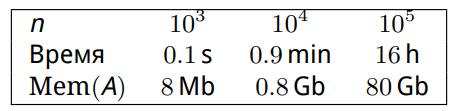
\includegraphics[width=0.6\textwidth, keepaspectratio]{../figs/svd_time.png}
			 		\end{figure}
			 		
			 		Для CPD-разложения всё также непросто. Несмотря на его хорошие свойства, вычисление канонического ранга $ r $ является NP-трудной задачей. Поэтому при  применении tSSA его необходимо подбирать. Из-за неточности этого подбора возможна большая ошибка аппроксимации исходного тензора $ \mathbf{T} $, а выбор больших $ r $ приводит к огромному времени вычисления и потребляемой памяти. Достаточно быстрый приближённый алгоритм ALS (Alternating Least Squares) всё равно оперирует матрицами, их свёртками и нахождениями минимума матричных функций, что катастрофично для тензоров больших размеров.
			 
			 \subsection*{Вычислительный эксперимент}
			 
			 
			 \subsection*{Выводы}
			
			
		
		\newpage
		\printbibliography
	
\end{document}